\chapter{Evaluation}
\label{chapter6}
Um die Praxistauglichkeit zu überprüfen, werden nun ausgewählte Daten
mithilfe des entwickelten Tools geclustert.
Die Ergebnisse werden anschließend bewertet.
Zur Bewertung des Clusterings werden \emph{externe}
und \emph{interne} Indizes unterschieden \citep{aghabozorgi_time-series_2015, warren_liao_clustering_2005}.
Bei einem \emph{externen Index} werden \emph{Ground-Truth-Daten} extern bereitgestellt.
Nach dem Clustering kann der Grad der Übereinstimmung zwischen gefundenen Clustern
und den vorgegebenen Clustern überprüft werden \citep{aghabozorgi_time-series_2015, warren_liao_clustering_2005}.
Die Daten werden mithilfe einer Visualisierung manuell geclustert.
In \autoref{6-GroundTruth} werden die gefundenen Cluster mit den erwarteten verglichen.
Bei \emph{internen Indizes} muss die Qualität der Cluster hingegen
ohne zusätzliche Informationen überprüft werden \citep{aghabozorgi_time-series_2015, warren_liao_clustering_2005}.
Dazu sollen in \autoref{6-Statistical} \emph{deskriptive Statistiken} genutzt werden.
Die Standardabweichung, der Mittelwert, das Maximum und das Minimum liefern
ein Maß für die Ähnlichkeit von Cluster-Komponenten.
Damit wird überprüft,
ob zusammengefasste Records tatsächlich einen hohen Grad an Übereinstimmung aufweisen.

\section{Einführende Bemerkungen}
\label{6-Bemerkungen}
Statt den gesamten, in \autoref{2-StrukturDatensatz} beschriebenen, Datensatz zu verwenden,
sollen geeignete Teilmengen genutzt werden.
Es wurde eine gefilterte Version des Datensatzes bereitgestellt.
Zu kurze oder fehlerhafte Records wurden aussortiert (\autoref{2-StrukturDatensatz}).
Außerdem erfolgte eine Sortierung nach Personenzahl.
Das Filtern der Daten gehört nicht zu den Anforderungen an das entwickelte Tool
und wird daher nicht in dieser Arbeit betrachtet.
Dennoch sollte dem Nutzer bewusst sein,
dass mit gefilterten Daten gegebenenfalls aussagekräftigere Ergebnisse erzielbar sind.
Gerade die separate Betrachtung von Records mit unterschiedlicher Personenzahl kann helfen,
wiederkehrende Bewegungsmuster durch Clustering zu erkennen.
In der Evaluation werden nur Records mit ein bis drei Personen betrachtet.

Ebenfalls zu erwähnen ist die Bedeutung eines geeigneten Threshold-Wertes für ein erfolgreiches Clustering.
Dieser kann je nach vorliegenden Daten, verwendeten Attributen und Zielstellung variieren.
Häufig ist daher ein {\glqq Herantasten\grqq} nötig.
In den später beschriebenen Szenarien war beispielsweise auffällig,
dass der Threshold bei Records mit einer Person deutlich niedriger war
als bei Records mit mehreren Personen.
Abhängig davon wie viele Cluster am Ende erwünscht sind
und wie stark die Cluster-Bestandteile voneinander abweichen dürfen,
muss ein anderer Wert gewählt werden.

Die Ground-Truth-Daten wurden manuell mithilfe der Visualisierung erstellt.
Zunächst werden drei Minimalbeispiele betrachtet.
Dafür wurden für die Fälle, eine bis drei Personen, jeweils beliebig 25 Records gewählt.
Diese wurden mithilfe des Visualizers und Kinect Studio visualisiert und manuell in Cluster eingeteilt.
\autoref{fig:Clusters} zeigt jeweils die Visualisierung eines Repräsentanten der Cluster.
\begin{figure}[ht]
    \begin{center}
    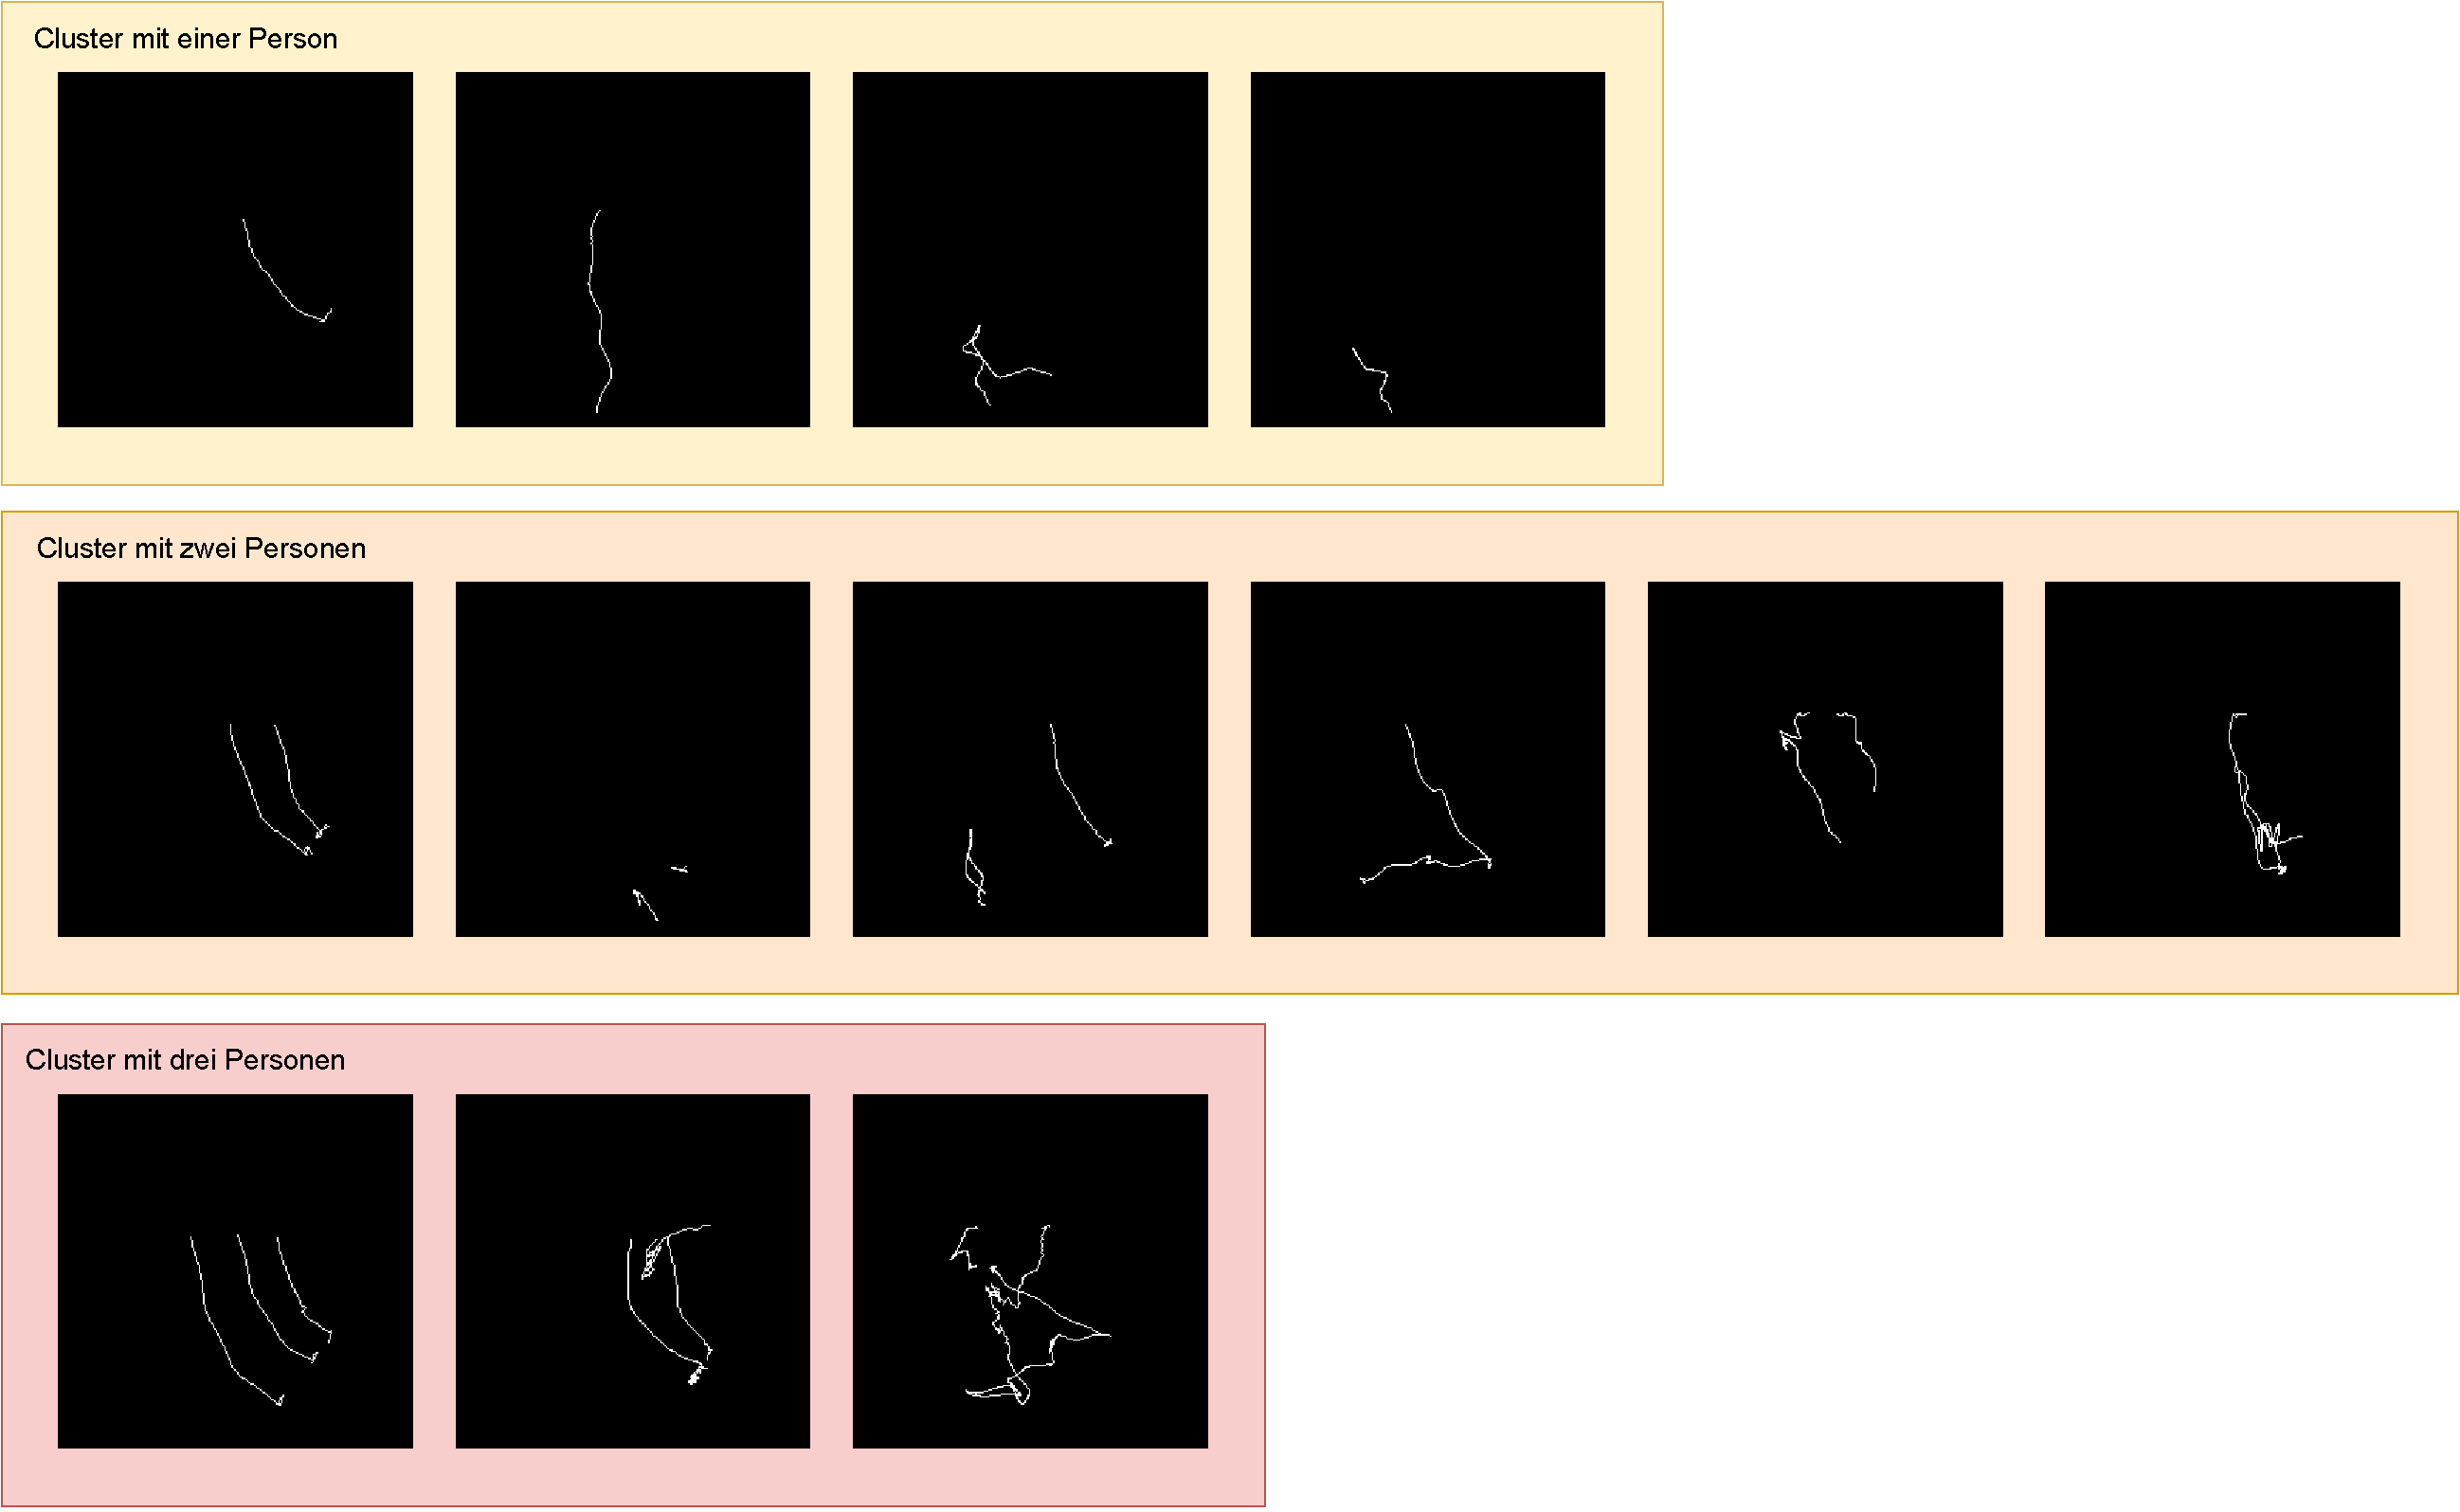
\includegraphics[width=1.2\textwidth, angle=90]{clusters.pdf}
    \end{center}
    \caption{Repräsentanten der manuell erstellten Cluster.}
    \label{fig:Clusters}
\end{figure}
Die Ergebnisse und eine sprachliche Beschreibung des Inhalts
können im Evaluation-Verzeichnis des Code-Repositories eingesehen werden.
Das hierarchische Clustering wurde mit den x- und z-Werten als Vergleichsattribute gestartet.
Der Threshold wurde dabei jeweils so gewählt,
dass genau so viele Cluster entstehen wie auch manuell erkannt wurden.
Die Auswertung zeigt, dass die vom Tool berechneten Cluster genau mit den Ground-Truth-Daten übereinstimmen.
Diese Minimalbeispiele sind aber nur bedingt aussagekräftig,
da lediglich eine kleine Teilmenge der tatsächlich vorhandenen Daten genutzt wurde.
Manche Muster treten dadurch gegebenenfalls überhaupt nicht auf.
In \autoref{6-GroundTruth} soll die Analyse daher auf größere Mengen gefilterter Daten,
für ein bis drei Personen, ausgeweitet werden.
Aufgrund der Vielzahl der Daten ist das manuelle Clustering allerdings nicht so
zuverlässig möglich wie in den oben beschriebenen Minimalbeispielen.
Die Daten wurden aber nach bestem Wissen, auf die wichtigsten Bewegungen hin, untersucht.
Spezielle Bewegungen, die nur einmalig auftreten, wurden ignoriert.
Ziel ist es zu überprüfen,
ob häufig wiederkehrende Muster korrekt vom Tool erkannt werden.
Abschließend bleibt zu erwähnen,
dass beim Clustering von Bewegungsdaten, mithilfe von Laufwegen,
der Zweck des Gehens offen bleibt \citep{monastero_traces_2018}.
Dieser kann durch manuelle Interpretation bestimmt werden,
wobei die gefundenen Cluster unterstützend eingesetzt werden können.
Zur Automatisierung derartiger Interpretationen ist weitere Forschung notwendig.

\section{Ground-Truth-Analyse}
\label{6-GroundTruth}
Im gefilterten Datensatz mit drei Personen befinden sich insgesamt 103 Records.
Die manuelle Einteilung ergab,
dass es sich bei vielen darin vorkommenden Bewegungsabläufen
um spezielle Bewegungen, die nicht häufiger auftreten, handelt.
Sie werden im Folgenden nicht aufgeführt.
Allerdings wurde ein eindeutiges Cluster identifiziert.
\autoref{fig:3PersClust1} zeigt einen Repräsentanten dieses Clusters.
\begin{figure}[ht]
    \begin{center}
    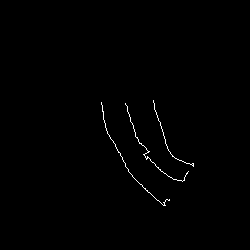
\includegraphics[width=0.15\textwidth]{representation3PersCluster1.png}
    \end{center}
    \caption{Repräsentant des nicht trivialen Clusters mit drei Personen.}
    \label{fig:3PersClust1}
\end{figure}
Es handelt sich dabei um drei Personen, die nebeneinander durch den Sensorbereich laufen.
Dieselben Erkenntnisse lieferte auch das Minimalbeispiel aus \autoref{6-Bemerkungen}.
Grund hierfür kann sein, dass die Datenmenge mit circa 100 Records immer noch gering ist.
Anschließend wurde überprüft, ob auch das Tool diese häufig auftretende Bewegung korrekt erkannt hat.
Die Ergebnisse der Berechnungen stimmen mit dem manuell gefundenen Cluster überein.
Im Wesentlichen wird nur ein nicht-triviales Cluster gefunden,
und zwar das oben beschriebene.

Die Teilmenge aller Records mit zwei Personen enthält 513 Records.
Bei der manuellen Durchsicht lassen sich wieder spezielle,
nicht wiederkehrende Bewegungen erkennen.
Diese werden erneut ignoriert.
Im Gegensatz zum Fall mit drei Personen sind hier aber mehrere häufig auftretende Bewegungen identifizierbar.
\autoref{fig:2PersClusters} zeigt jeweils einen Repräsentanten dieser manuell erkannten Muster.
\begin{figure}[ht]
    \begin{center}
    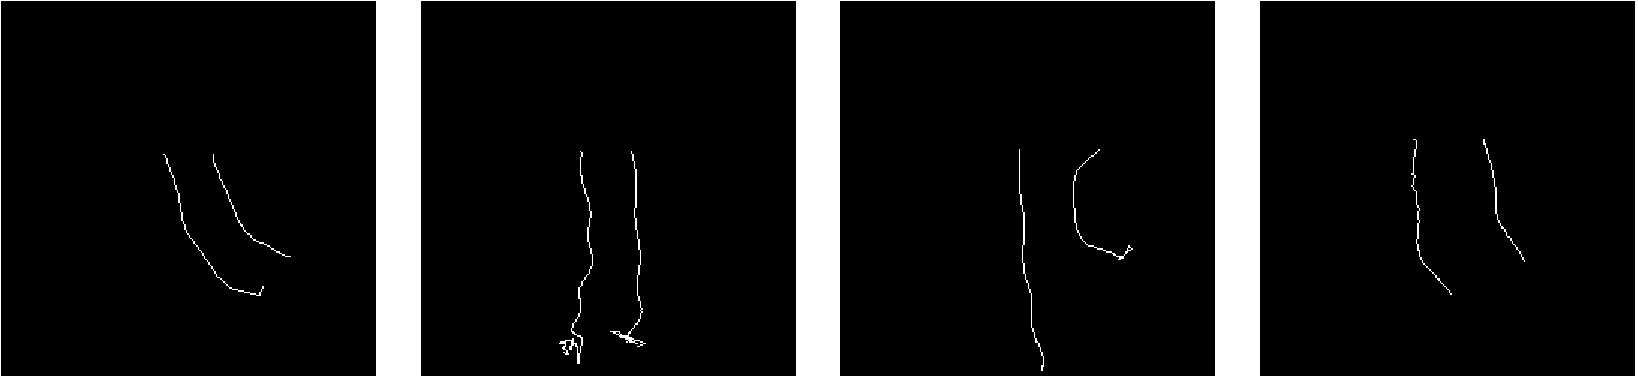
\includegraphics[width=0.65\textwidth]{2PersClusters.pdf}
    \end{center}
    \caption{Repräsentanten der größten Cluster mit zwei Personen.}
    \label{fig:2PersClusters}
\end{figure}
Zum einen handelt es sich um den Fall, dass zwei Personen durch den Aufnahmebereich laufen.
Dies ist die analoge Bewegung zum gefundenen Cluster bei drei Personen.
Der zweite Fall zeigt, wie sich zwei Personen dem Sensor nähern.
In Szenario drei bewegt sich eine Person zur Kamera,
während eine andere lediglich durch das Bild läuft.
Im letzten Fall laufen zwei Personen gemeinsam zum oberen Bildrand.
Alle Szenarien werden durch das Tool gefunden.
Bei dieser großen Menge an Records fällt auf,
dass bei niedrigen Thresholds ähnliche Records teilweise noch in unterschiedlichen Clustern liegen
und erst in späteren Schritten kombiniert werden,
da andere Szenarien noch eine höhere Ähnlichkeit aufweisen.

Das Tool kann für Datensätze mit Ein- bis Zweitausend Records effizient eingesetzt werden.
Auf einem heute typischen Mittelklasse-Heimrechner werden innerhalb weniger Minuten Ergebnisse geliefert.
Ab einigen Tausend Records nimmt die Bearbeitungszeit zu,
sodass, unter Umständen, mit mehreren Stunden Wartezeit zu rechnen ist.
Die meisten hierarchischen Clustering-Verfahren werden den Komplexitätsklassen
\emph{O(n²)} oder \emph{O(n³)} zugeordnet.
Das implementierte Tool fällt in die Klasse \emph{O(n²)},
wie die Zeitmessungen aus \autoref{tbl:CalcTime} belegen.
Die Verdoppelung der Recordanzahl führt nicht zu einer Verachtfachung der Bearbeitungszeit,
wie dies bei \emph{O(n³)} der Fall wäre.
Die Zeit zum Einlesen der Daten
und zum Schreiben der Ergebnisse wurde hier ignoriert.
\begin{table}[ht]
  \begin{center}
  \begin{tabular}{ |c|c| } 
   \hline
   Recordanzahl & Bearbeitungszeit (Sekunden) \\
   \hline \hline
   100 & 9 \\
   \hline
   200 & 30 \\
   \hline
   400 & 133 \\
   \hline
   800 & 637 \\
   \hline
  \end{tabular}
  \caption{Bearbeitungszeiten des Clusteringvorgangs nach Recordanzahl.}
  \label{tbl:CalcTime}
  \end{center}
\end{table}
Diese Limitierung muss beachtet werden,
falls in Zukunft noch umfangreichere Datenmengen geclustert werden müssen.
In diesem Fall muss entweder ein leistungsstärkerer Rechner eingesetzt
oder das Tool weiter optimiert werden.
Mögliche Optionen sind Parallelisierung
oder die Implementierung einer effizienteren Version des Clustering-Verfahrens \citep{patel_study_2015}.

Insgesamt befinden sich 3523 Records mit einer Person im gefilterten Datensatz.
Allerdings wiederholen sich die Bewegungsmuster oft.
Deshalb soll die Analyse im Folgenden auf eine Teilmenge mit 1000 beliebigen Records eingeschränkt werden.
Erneut wird überprüft, ob wiederkehrende Bewegungen korrekt erkannt werden.
\autoref{fig:1PersClusters} zeigt jeweils einen Repräsentanten der manuell erkannten Muster.
\begin{figure}[ht]
    \begin{center}
    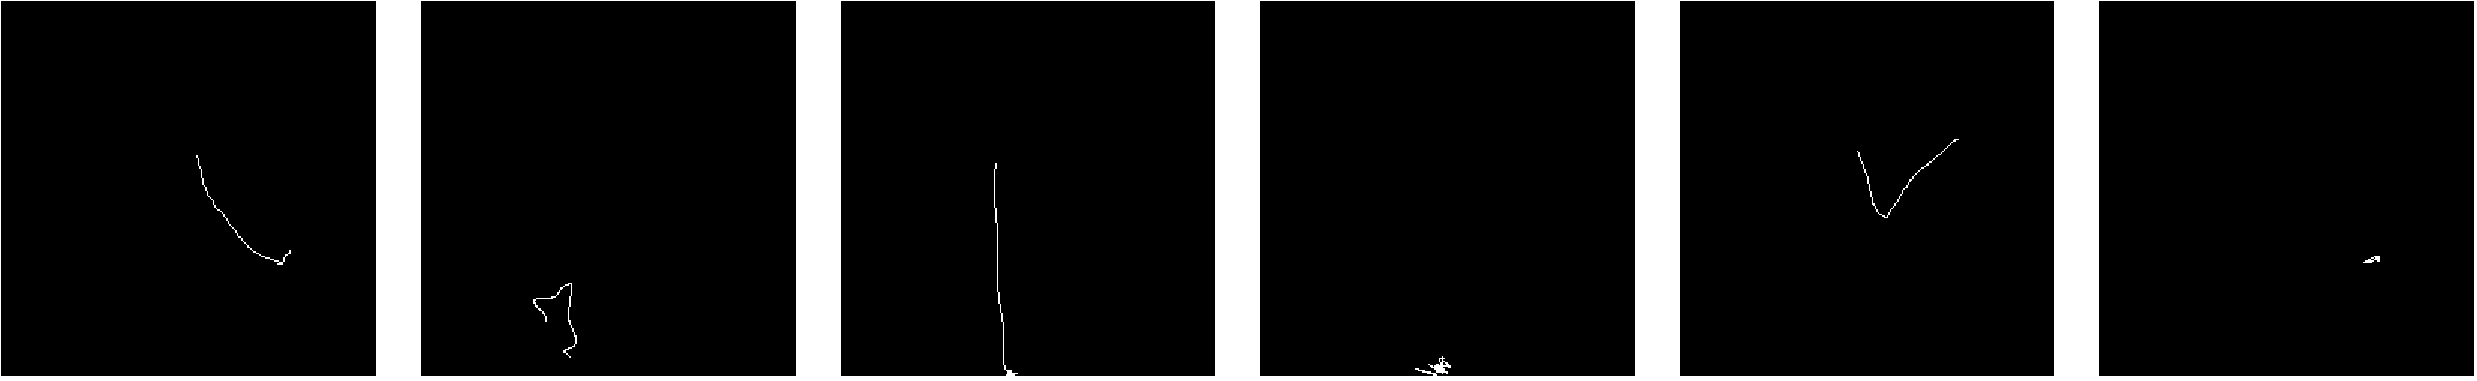
\includegraphics[width=\textwidth]{1PersClusters.pdf}
    \end{center}
    \caption{Repräsentanten der größten Cluster mit einer Person.}
    \label{fig:1PersClusters}
\end{figure}
Im ersten Fall bewegt sich eine Person durch den Aufnahmebereich,
während sie sich im zweiten Szenario unmittelbar vor der Kamera befindet.
Bild drei zeigt ein direktes Zugehen auf den Bildschirm.
Im vierten und sechsten Fall steht die Person an verschiedenen Positionen beinahe still.
Szenario fünf zeigt, wie eine Person nach vorne läuft,
sich umdreht und wieder zurückläuft.
All diese Fälle können durch das Tool erkannt werden.
Zu erwähnen ist allerdings, dass manche Cluster bei hohen Thresholds bereits in andere Gruppen integriert werden.
So kann etwa das fünfte Szenario nur bei niedrigeren Thresholds erkannt werden,
während es bei höheren Werten unter Umständen bereits mit Cluster eins zusammengeführt wurde.
Dies verdeutlicht erneut, dass eine sinnvolle Suche nach Clustern möglich ist,
diese aber dennoch manuell betrachtet werden müssen.
Dabei sollte auch mit verschiedenen Thresholds experimentiert werden.

Die Auswertung des gesamten Datensatzes bestätigt demnach die Vermutung der Minimalbeispiele.
Das Tool kann genutzt werden, um sinnvolle Cluster in den Kinect-Bewegungsdaten zu finden.
Im folgenden Abschnitt soll abschließend die Güte der gefundenen Cluster an einigen Beispielen
überprüft werden.

\section{Statistische Analyse}
\label{6-Statistical}
Abschließend soll mithilfe von deskriptiven Statistiken überprüft werden,
ob ein qualitativer Zusammenhang zwischen den Record-Bestandteilen eines Clusters besteht.
Der Grad der Übereinstimmung liefert Informationen zur Ähnlichkeit.
Konkret werden nun für die Komponenten einiger Cluster
die Standardabweichung, der Mittelwert, das Maximum und das Minimum für die x-Laufwege berechnet
und tabellarisch dargestellt.
In der letzten Zeile ist jeweils die Standardabweichung aller darüberstehenden Werte aufgeführt.
Hier werden teilweise die Minimalbeispiele aus \autoref{6-GroundTruth}, mit veränderten Thresholds, wieder aufgegriffen.
Auch diese Daten befinden sich im Evaluation-Verzeichnis des Code-Repositories.
Zunächst wird das erste Cluster mit drei Personen betrachtet (\autoref{fig:Clusters}).
Die Ergebnisse werden in \autoref{tbl:ClustThreePers} dargestellt
und sind auf zwei Nachkommastellen gerundet.
Anschließend werden die Werte des ersten Clusters mit zwei Personen aus \autoref{fig:Clusters} berechnet.
Sie sind in \autoref{tbl:ClustTwoPers} zu sehen.
Wird im selben Beispiel der Threshold noch höher gesetzt,
sodass die gefundenen Cluster augenscheinlich nicht mehr sinnvoll sind,
werden die Werte in \autoref{tbl:ClustTwoPersHighThreshold} geliefert.
\begin{table}[ht]
  \begin{center}
    \begin{tabular}{ |c|c|c|c|c| } 
      \hline
      Record & Minimum & Maximum & Mittelwert & Standardabw. \\
      \hline \hline
      2017-05-04 16.35.15.463 & -2.12 & 0.63 & -0.59 & 0,72 \\
      \hline
      2017-04-13 12.34.38.535 & -1.72 & 0.46 & -0.65 & 0,58 \\
      \hline
      2017-05-08 12.30.56.954 & -2.09 & 0.12 & -1.01 & 0.56 \\
      \hline
      2017-04-13 12.36.06.669 & -1.83 & 0.43 & -0.70 & 0.57 \\
      \hline
      2017-04-20 12.35.56.578 & -2.06 & 0.50 & -0.75 & 0.67 \\
      \hline
      2017-04-10 11.53.16.991 & -2.09 & -0.61 & -1.15 & 0.36 \\
      \hline
      2017-05-08 12.45.55.652 & -1.84 & 0.51 & -0.64 & 0.65 \\
      \hline
      2017-04-06 09.47.43.189 & -1.96 & 0.44 & -0.66 & 0.64 \\
      \hline
      2017-04-05 13.00.04.745 & -1.79 & 0.17 & -0.79 & 0.50 \\
      \hline
      2017-04-11 13.29.55.196 & -2.06 & 0.72 & -0.47 & 0.72 \\
      \hline
      2017-04-07 13.19.05.395 & -2.01 & 0.32 & -0.81 & 0.56 \\
      \hline
      2017-04-21 14.17.23.301 & -2.03 & 0.30 & -0.91 & 0.59 \\
      \hline
      2017-04-26 11.59.37.413 & -1.74 & 0.31 & -0.76 & 0.55 \\
      \hline
      2017-04-21 12.58.27.894 & -1.84 & 0.20 & -0.81 & 0.51 \\
      \hline
      2017-04-19 12.54.19.390 & -1.81 & 0.66 & -0.54 & 0.69 \\
      \hline
      2017-04-27 12.36.45.995 & -1.85 & -0.04 & -0.92 & 0.50 \\
      \hline
      2017-05-04 13.13.17.884 & -2.07 & -0.03 & -0.85 & 0.52 \\
      \hline
      2017-04-05 09.28.25.562 & -1.78 & 0.36 & -0.66 & 0.58 \\
      \hline
      2017-05-04 13.24.36.117 & -2.00 & 0.38 & -0.66 & 0.65 \\
      \hline
      2017-04-05 13.01.44.147 & -2.20 & 0.41 & -0.73 & 0.63 \\
      \hline
      2017-04-07 11.05.51.351 & -1.89 & 0.32 & -0.63 & 0.65 \\
      \hline
      \hline
      Standardabweichung & 0.14 & 0.29 & 0.16 & 0.09 \\
      \hline
    \end{tabular}
    \caption{Deskriptive Statistiken für das Cluster mit drei Personen.}
    \label{tbl:ClustThreePers}
  \end{center}
\end{table}
  \begin{table}[ht]
    \begin{center}
      \begin{tabular}{ |c|c|c|c|c| } 
        \hline
        Record & Minimum & Maximum & Mittelwert & Standardabw. \\
        \hline \hline
        2017-04-06 12.26.06.199 & -1.90 & -0.34 & -0.98 & 0,49 \\
        \hline
        2017-04-05 09.13.53.631 & -1.73 & 0.01 & -0.88 & 0,41\\
        \hline
        2017-04-04 16.54.30.868 & -1.67 & 0.45 & -0.61 & 0.61 \\
        \hline
        2017-04-05 12.32.59.075 & -1.71 & 0.30 & -0.62 & 0.54 \\
        \hline
        2017-04-05 12.53.33.743 & -1.80 & 0.28 & -0.67 & 0.55 \\
        \hline
        2017-04-05 10.03.28.598 & -1.89 & -0.02 & -1.00 & 0.51 \\
        \hline
        2017-04-05 08.16.53.128 & -1.77 & -0.03 & -0.88 & 0.48 \\
        \hline
        2017-04-05 14.44.27.088 & -1.87 & 0.31 & -0.72 & 0.60 \\
        \hline
        2017-04-06 12.31.41.933 & -1.77 & 0.28 & -0.70 & 0.61 \\
        \hline
        2017-04-05 15.01.29.988 & -1.95 & 0.58 & -0.50 & 0.68 \\
        \hline
        2017-04-04 17.27.46.240 & -1.93 & -0.32 & -1.10 & 0.38 \\
        \hline
        2017-04-05 15.02.00.252 & -2.13 & 0.26 & -0.83 & 0.65 \\
        \hline
        2017-04-05 17.08.48.758 & -1.76 & 0.30 & -0.73 & 0.64 \\
        \hline
        2017-04-05 16.59.22.830 & -1.92 & 0.38 & -0.74 & 0.57 \\
        \hline
        2017-04-05 11.40.51.237 & -1.32 & 0.17 & -0.49 & 0.46 \\
        \hline
        2017-04-06 11.38.42.632 & -1.67 & 0.12 & -0.81 & 0.50 \\
        \hline
        2017-04-05 10.56.51.141 & -1.77 & 0.31 & -0.68 & 0.58 \\
        \hline
        2017-04-05 12.29.05.007 & -1.85 & 0.16 & -0.80 & 0.55 \\
        \hline
        2017-04-05 13.33.56.412 & -1.97 & 0.31 & -0.79 & 0.63 \\
        \hline
        2017-04-05 10.59.42.469 & -1.77 & -0.17 & -0.92 & 0.49 \\
        \hline
        \hline
        Standardabweichung & 0.16 & 0.24 & 0.16 & 0.08 \\
        \hline
       \end{tabular}
    \caption{Deskriptive Statistiken für das Cluster mit zwei Personen.}
    \label{tbl:ClustTwoPers}
  \end{center}
\end{table}
\begin{table}[ht]
  \begin{center}
    \begin{tabular}{ |c|c|c|c|c| } 
      \hline
      Record & Minimum & Maximum & Mittelwert & Standardabw. \\
      \hline \hline
      2017-04-06 12.26.06.199 & -1.90 & -0.34 & -0.98 & 0,49 \\
      \hline
      2017-04-05 09.13.53.631 & -1.73 & 0.01 & -0.88 & 0,41\\
      \hline
      2017-04-04 16.54.30.868 & -1.67 & 0.45 & -0.61 & 0.61 \\
      \hline
      2017-04-05 12.32.59.075 & -1.71 & 0.30 & -0.62 & 0.54 \\
      \hline
      2017-04-04 18.04.06.507 & -1.23 & 1.07 & -0.14 & 0.54 \\
      \hline
      2017-04-05 12.53.33.743 & -1.80 & 0.28 & -0.67 & 0.55 \\
      \hline
      2017-04-05 10.03.28.598 & -1.89 & -0.02 & -1.00 & 0.51 \\
      \hline
      2017-04-05 08.16.53.128 & -1.77 & -0.03 & -0.88 & 0.48 \\
      \hline
      2017-04-05 12.40.57.142 & -1.52 & -0.23 & -1.00 & 0.22 \\
      \hline
      2017-04-05 14.44.27.088 & -1.87 & 0.31 & -0.72 & 0.60 \\
      \hline
      2017-04-06 12.31.41.933 & -1.77 & 0.28 & -0.70 & 0.61 \\
      \hline
      2017-04-05 15.01.29.988 & -1.95 & 0.58 & -0.50 & 0.68 \\
      \hline
      2017-04-04 17.27.46.240 & -1.93 & -0.32 & -1.10 & 0.38 \\
      \hline
      \textbf{2017-04-04 14.55.11.727} & \textbf{-1.57} & \textbf{1.02} & \textbf{0.36} & \textbf{0.84} \\
      \hline
      2017-04-05 15.02.00.252 & -2.13 & 0.26 & -0.83 & 0.65 \\
      \hline
      2017-04-05 17.08.48.758 & -1.76 & 0.30 & -0.73 & 0.64 \\
      \hline
      2017-04-05 16.59.22.830 & -1.92 & 0.38 & -0.74 & 0.57 \\
      \hline
      2017-04-05 11.40.51.237 & -1.32 & 0.17 & -0.49 & 0.46 \\
      \hline
      2017-04-05 11.41.21.472 & -1.08 & -0.14 & -0.53 & 0.36 \\
      \hline
      2017-04-06 11.38.42.632 & -1.67 & 0.12 & -0.81 & 0.50 \\
      \hline
      2017-04-05 10.56.51.141 & -1.77 & 0.31 & -0.68 & 0.58 \\
      \hline
      2017-04-05 12.29.05.007 & -1.85 & 0.16 & -0.80 & 0.55 \\
      \hline
      2017-04-05 13.33.56.412 & -1.97 & 0.31 & -0.79 & 0.63 \\
      \hline
      2017-04-05 10.59.42.469 & -1.77 & -0.17 & -0.92 & 0.49 \\
      \hline
      \hline
      Standardabweichung & 0.24 & 0.35 & 0.31 & 0.12 \\
      \hline
     \end{tabular}
    \caption{Deskriptive Statistiken für das Cluster mit zwei Pers. (hoher Threshold).}
    \label{tbl:ClustTwoPersHighThreshold}
  \end{center}
\end{table}
Die Mittelwerte und Standardabweichungen in den ersten beiden Beispielen
bewegen sich jeweils in einem ähnlichen Rahmen.
Auch die Standardabweichung dieser Werte ist mit \emph{0.16} und \emph{0.09} im ersten,
sowie \emph{0.16} und \emph{0.08} im zweiten überprüften Cluster gering.
Dadurch wird bestätigt, dass die Records einen inhaltlichen Zusammenhang aufweisen.
Beim dritten Fall hingegen schwanken diese Werte stärker.
Die ermittelte Gesamtstandardabweichungen sind mit \emph{0.31} und \emph{0.12} um
circa 52 Prozent, bzw. 39 Prozent höher als bei den zuerst betrachteten Clustern.
Einige Records scheinen also nicht in die Gruppe zu passen.
So weicht beispielsweise die Zeile \emph{2017-04-04 14.55.11.727} stark von den anderen ab.
Ein Blick in die Visualisierung bestätigt,
dass dieser Laufweg nicht zu den anderen passt.
Dieser Fall wurde lediglich aufgrund des zu hohen Thresholds einsortiert.
Dies betont einerseits erneut die bedeutende Rolle eines geeigneten Thresholds
und andererseits, dass die Bestimmung der Güte mittels deskriptiver Statistiken möglich ist.
Die Records der Cluster der beiden ersten Beispiele weisen eine hohe Ähnlichkeit auf.
Mithilfe des entwickelten Tools ist folglich ein sinnvolles Clustering möglich.
Beim letzten Cluster sind durch einen hohen Threshold hingegen zu viele Records zusammengeführt worden.